\chapter{Desarrollo del trabajo}

En este capítulo se realizará un estudio detallado del estado del arte para posteriormente detallar las distintas fases de desarrollo y los problemas que han surgido con sus respectivas soluciones.

\section{Desarrollo profundo del estado del arte}

Este trabajo es la continuación de mi anteior TFG donde traté el tema de la renderización de conjuntos de datos volumétricos, este trabajo está dirigido al tratamiento de este conjunto de datos.

Un conjunto de datos volumétrico o campo escalar 3D está representado por una función $R^{3} \rightarrow R$. En otras palabras, se trata de un conjunto de datos representado por una matriz tridimensional, donde cada elemento de esta matriz se puede denominar vóxel y es importante tener claro que el valor de este no es un color sino un valor como tal que posteriormente se renderizará con un color y una transparencia según una función de transferencia. Es ahí donde erradica la separación conceptual entre modelado y visualización de un conjunto de datos volumétrico.

El flujo a la hora de representar un conjunto de datos volumétricos sería el siguiente:

\begin{itemize}
	\item Obtención de imágenes
	\item Filtrado
	\item Segmentación
	\item Visualización
\end{itemize}

Durante el TFG traté el último de los pasos y en este TFM comentaré las distintas opciones del primero y trabajaré en técnicas del segundo y el tercero aplicadas a esculturas de madera policromadas.

\subsection{Obtención de imágenes}

Existen diversas técnicas de obtención de imágenes volumétricas. En esta sección se describirán las dos técnicas más usadas actualmente y se realizará una comparación entre ellas. No se han incluido técnicas como el PET, SPECT o ecografía pues necesitan de contrastes que no se podrían aplicar en una escultura si se quiere preservar su estado.

\subsubsection{Tomografía Computarizada}

La Tomografía Computarizada (TC o CT en inglés) fue la primera de las técnicas que surgió para la obtención de datos volumétricos pero ha ido evolucionando hasta el día de hoy como se detalló en la introducción.

\begin{figure}[H]
	\centering
	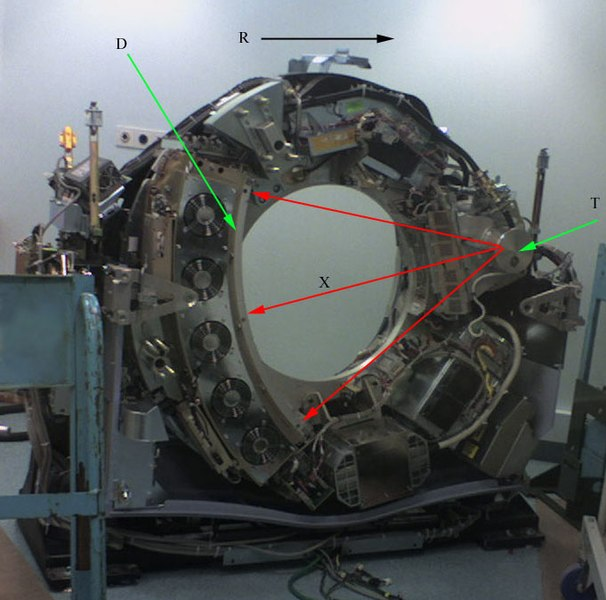
\includegraphics[width=9cm]{imagenes/desarrollo/tc}
	\caption{Escáner TC sin la carcasa, por lo que se puede ver sus componentes internos. T: Tubo rayos X, D: Detectores rayos X, X: Haces de rayos X y R: \textit{Gantry}. Imagen extraída de: \url{https://en.wikipedia.org/wiki/File:Ct-internals.jpg}}
	\label{fig:desarrollo/tc}
\end{figure}

Los parámetros utilizados en una TC son los siguientes:

\begin{itemize}
	\item \textbf{Resolución espacial} (número de cortes, píxeles por corte y distancia entre vóxeles): Si la resolución es más alta los datos serán más ruidosos si la dosis de radiación se mantiene.
	\item \textbf{Dosis de radiación}: Si la dosis de radiación es mayor se conseguirá mejor ratio señal-ruido y las imágenes podrán ser de mayor resolución sin que el ruido sea un problema.
	\item \textbf{\textit{Gantry tilt}} (sistema de rotación emisor/receptor): Se puede adaptar el \textit{gantry tilt} para una parte específica a examinar.
\end{itemize}

Los valores de intensidad de las imágenes extraídas se encuentran en unidades Hounsfield (HU). Que es una unidad de medida normalizada que hace que un tejido tenga ese valor sean cuales sean los parámetros del escáner.

\subsubsection{Imagen por Resonancia Magnética}

La Imagen por Resonancia Magnética (IRM o MRI en inglés) es una técnica en la que, a diferencia de la TC donde se usa radiación ionizante, se usan campos mágnéticos para diferenciar los distintos materiales del objeto escaneado, específicamente la ocurrencia del núcleo de hidrógeno que son capaces de absorber y emitir radio frecuencia cuando se colocan en un campo magnético externo \cite{mcrobbie10}.

\begin{figure}[H]
	\centering
	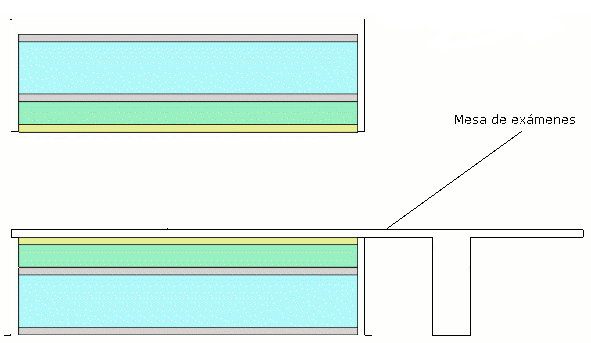
\includegraphics[width=12cm]{imagenes/desarrollo/irm-longitudinal}
	\caption{Esquema de un escáner IRM (Sección Longitudinal). Imagen extraída de: \url{https://en.wikipedia.org/wiki/File:Mri_scanner_schematic_labelled.svg}}
	\label{fig:desarrollo/irm-longitudinal}
\end{figure}

\begin{figure}[H]
	\centering
	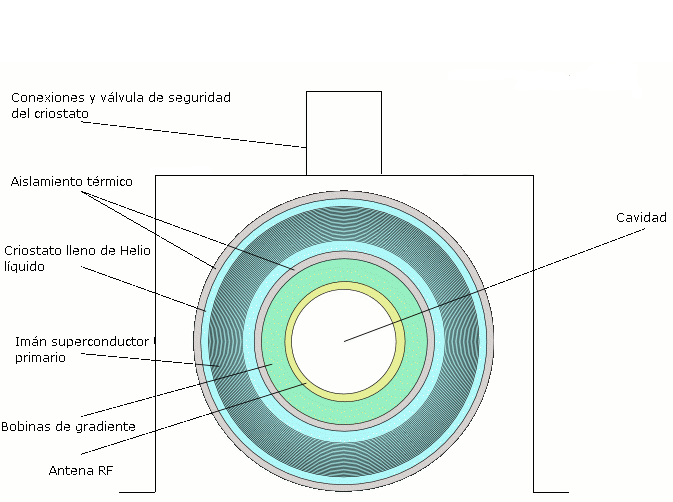
\includegraphics[width=12cm]{imagenes/desarrollo/irm-axial}
	\caption{Esquema de un escáner IRM (Sección Axial). Imagen extraída de: \url{https://en.wikipedia.org/wiki/File:Mri_scanner_schematic_labelled.svg}}
	\label{fig:desarrollo/irm-axial}
\end{figure}

El campo magnético alinea los momentos magnéticos de los núcleos atómicos de hidrógeno en dirección paralela y anti-paralela. 

A continuación se emite radiación electromagnética a un pulso de radiofrecuencia determinado. Algunos núcleos que se encuentran en dirección paralela pasarán a anti-paralela y al volver a su dirección original perderán energía en forma de fotones que podrán ser detectados. 

Estos dos tiempos, T1 (\textit{phase}) y T2 (\textit{dephase}) son medidos. Para obtener T1 hay que ver el valor en la gráfica de relajación longitudinal al 63\% y para obtener T2 hay que hacer lo mismo en la gráfica de relajación transversal al 37\% \cite{relaxation}.

\begin{figure}[H]
	\centering
	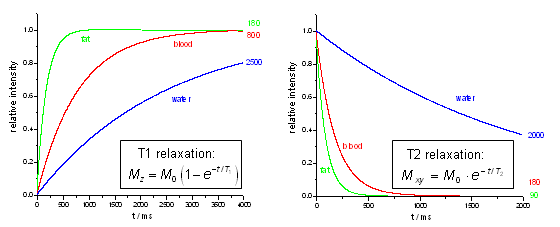
\includegraphics[width=12cm]{imagenes/desarrollo/relajacion-longitudinal-transversal}
	\caption{A la izquierda gráfica de la relajación longitudinal (crecimiento logarítmico) y a la derecha gráfica de la relajación transversal (crecimiento exponencial) \cite{relaxation}}
	\label{fig:desarrollo/relajacion-longitudinal-transversal}
\end{figure}

\subsubsection{Comparación entre TC e IRM}

Las principales diferencias entre ambas técnicas son las siguientes:

\begin{itemize}
	\item La IRM obtiene imágenes de menor resolución que la TC.
	\item La IRM proporciona un mayor contraste entre tejidos poco densos.
	\item Los datos obtenidos con una TC son más entendibles por médicos mientras que los obtenidos con una IRM por radiólogos.
	\item El tiempo y coste de escaneo de una IRM es mayor que el de una TC.
	\item Los datos obtenidos con una TC se encuentran en unidades normalizadas mientras que los obtenidos con una IRM variarán dependiendo de los parámetros del escáner.
\end{itemize}

Al necesitar unos \textit{presets} con los que se pueda visualizar la escultura sin necesidad de que el usuario edite la función de transferencia, el último punto nos haría decantar por la TC. Además gracias a esta podremos obtener imágenes de mayor resolución. El único punto en contra en esta elección es que el contraste entre materiales de baja densidad (como la madera) no será tan distinguible como con la IRM.

\subsection{Filtrado}

Los datos en crudo obtenidos con las técnicas anteriormente descritas muchas veces no son lo suficientemente buenas y tienen lo que se denomina ruido. Hay muchos tipos de ruido y existen distintos filtros que aplicar a las imágenes para reducirlo.

Antes de describir los filtros más usados, se va a profundizar en ciertos aspectos teóricos necesarios para entender mejor cómo funcionan. Estos conceptos se van a describir para un espacio 2D, aunque pasar a un espacio 3D como el de los volúmenes es trivial pues tan solo haría falta utilizar una variable más para la profundidad.

Lo primero que hay que comprender es el concepto de vecindario. Que no es más que los píxeles que lo rodean a una distancia concreta. Por ejemplo un vecindario de tamaño 3x3 sobre el punto $p$ es un conjunto de píxeles con tamaño 3x3 con centro en el píxel $p$ (Figura \ref{fig:desarrollo/vecindario}).

\begin{figure}[H]
	\centering
	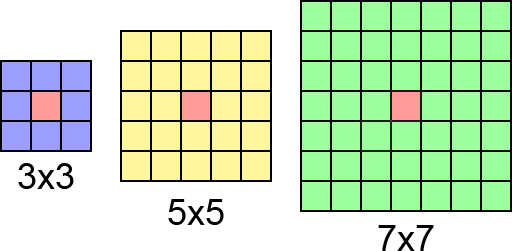
\includegraphics[width=10cm]{imagenes/desarrollo/vecindario}
	\caption{Vecindarios 3x3, 5x5 y 7x7 de un píxel (rojo).}
	\label{fig:desarrollo/vecindario}
\end{figure}

Un dominio espacial se denota con la expresión:

\[ g(x, y) = T[f(x, y)] \]

Donde:

\begin{itemize}
	\item $f(x, y)$ es la imagen de entrada
	\item $g(x, y)$ es la imagen de salida
	\item $T$ es un operador en $f$ definido sobre el vecindario $(x,y)$
\end{itemize}

Los filtros espaciales consisten en aplicar el operador $T$ a los píxeles del vecindario. Por ejemplo en un vecindario 3x3 y un operador $T$ definido como la intensidad media del vecindario, el valor $g(x_{i}, y_{j})$ será la suma del valor $f(x_{i}, y_{j})$ de su vecindario dividido entre 9.

\subsubsection{Filtro media}

El filtro media es el definido anteriormente. Es decir, usa un \textit{kernel} en el que todos los vecinos tienen el mismo peso.

Es un filtro utilizado para suavizar imágenes con mucho ruido.

\subsubsection{Filtro mediana}

El filtro media hace uso de la mediana para calcular el valor de salida del píxel. Por ejemplo, para la matriz: 

\[
\begin{bmatrix}
	1 & 4 & 0 \\
	2 & 2 & 4 \\
	1 & 0 & 1 
\end{bmatrix} 
\]

El valor para el punto $p$ correspondiente a $M(1, 1)$ con valor original 2, sería 1. Porque es la mediana de su vecindario (0, 0, 1, 1, \textbf{1}, 2, 2, 4, 4).

Este filtro es muy usado por ser el más efectivo para reducir el ruido de tipo \textit{salt-and-pepper} 

\begin{figure}[H]
	\centering
	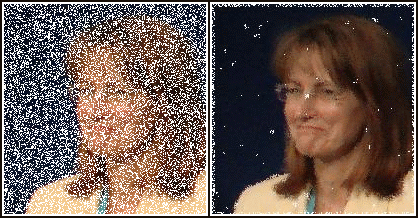
\includegraphics[width=11cm]{imagenes/desarrollo/salt-and-pepper}
	\caption{Ejemplo de ruido tipo \textit{salt-and-pepper}, utilizando un filtro mediana.  Imagen extraída de: \url{https://en.wikipedia.org/wiki/File:Medianfilterp.png}}
	\label{fig:desarrollo/salt-and-pepper}
\end{figure}

\subsubsection{Filtro \textit{gaussiano}}

El filtro \textit{gaussiano} o binomial (Figura \ref{fig:desarrollo/filtro-gaussiano}) hace uso de una versión discretizada de la función \textit{gaussiana} y, por tanto, se basa en la convolución de una matriz que para un vecindario 5x5 sería:

\[
\begin{bmatrix}
	1 & 4 & 6 & 4 & 1 \\
	4 & 16 & 24 & 16 & 4 \\
	6 & 24 & 36 & 24 & 6 \\
	4 & 16 & 24 & 16 & 4 \\
	1 & 4 & 6 & 4 & 1
\end{bmatrix} 
\]

Para normalizar los elementos del \textit{kernel} haría falta que sumasen 1, por lo que se divide entre la suma de todos sus elementos (256 en el caso de 5x5).

\begin{figure}[H]
	\centering
	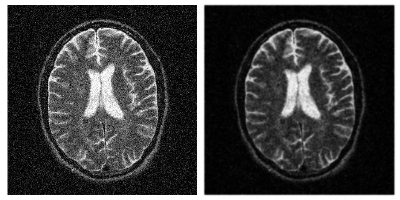
\includegraphics[width=11cm]{imagenes/desarrollo/filtro-gaussiano}
	\caption{Ejemplo de suavizado usado un fitro \textit{gaussiano}}
	\label{fig:desarrollo/filtro-gaussiano}
\end{figure}

Este filtro, al igual que el que hace uso de la media es, es un filtro paso baja utilizado para suavizar imágenes.

\subsection{Segmentación}

La segmentación es la separación de partes de un volumen para su estudio por separado. Antes de profundizar en algunas de las técnicas utilizadas en la actualidad, hay que tener claro una serie de conceptos \cite{segmentation-concepts}.

\begin{itemize}
	\item \textbf{Adyacencia}: Dos píxel son adyacentes si son vecinos y satisfacen un criterio de similitud, por ejemplo, que su valor de intensidad esté entre -700 y -300.
	\item \textbf{Camino}: Un camino entre dos píxeles es una secuencia de píxeles adyacentes que va desde un píxel hasta otro.
	\item \textbf{Conectividad}: Existe conectividad entre dos píxeles si se puede trazar al menos un camino entre ambos.
	\item \textbf{Componente conectado en un subconjunto de una imagen}: En un subconjunto $S$ de una imagen, para todos los píxeles $p$ en $S$, el conjunto de píxeles en $S$ conectados a $p$ se denominan componentes conectados en $S$.
	\item \textbf{Conjunto conectado}: Si el subconjunto de una imagen $S$ solo tiene un componente conectado, entonces se convierte en un conjunto conectado.
	\item \textbf{Región}: Un subconjunto $S$ de una imagen es una región si es un conjunto conectado.
	\item \textbf{Borde}: El borde de una región $S$ es el conjunto de píxeles que tienen uno o más vecinos no pertenecientes a $S$.
\end{itemize}

La segmentación trata de buscar los vóxeles que pertenecen a una estructura. Existen distintas aproximaciones como se detallaron en la introducción. A continuación se detallarán algunos de los métodos que se citaron.

\subsubsection{Segmentación basada en umbrales}

Esta segmentación es muy básica y trata de diferenciar las regiones utilizando dos umbrales de valor de intensidad y realizando un filtro en el que se descartasen todos aquellos vóxeles que no se encuentran entre estos valores \cite{otsu79}.

El uso de los histogramas de valores de la imagen pueden resultar útiles a la hora de seleccionar los umbrales.

Este método puede resultar útil para separar materiales con diferencias notables entre valores de densidad. En nuestro caso podría servir para separar madera de estuco, por ejemplo.

\subsubsection{Segmentación basada en crecimiento usando umbrales}

La segmentación basada en crecimiento usando umbrales es una extensión del método anterior, con la diferencia de que la segmentación basada en umbrales obtiene todas las regiones que se encuentran en la imagen y en la basada en crecimiento solo obtiene una región, obteniendo todos los puntos conectados a uno inicial que tienen el umbral como criterio de similitud \cite{haralick85} (Figura \ref{fig:desarrollo/segmentacion-crecimiento-umbral}).

\begin{figure}[H]
	\centering
	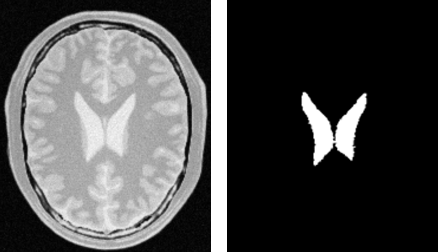
\includegraphics[width=11cm]{imagenes/desarrollo/segmentacion-crecimiento-umbral}
	\caption{Segmentación de los plexos coirodeos de una imagen de un cerebro usando una segmentación basada en crecimiento usando un umbral entre 210 y 255}
	\label{fig:desarrollo/segmentacion-crecimiento-umbral}
\end{figure}

Una variante de este método sería usar umbrales dinámicos. Es decir, en lugar de utilizar un valor máximo y mínimo global para toda la imagen (por ejemplo, valores de densidad entre -700 y -300), usar un rango dependiendo del punto donde se encuentro (por ejemplo, si el rango es de 100 y estamos en un punto con valor -532, el umbral para sus vecinos estaría entre -632 y -432). Este es el método de segmentación que se implementó en el TFG para segmentar las piezas separadas de la escultura como los elementos de la camilla.

En este caso es muy importante elegir el punto inicial, pues si se escoge un punto que se encuentre cercano al borde, puede hacer que la segmentación se extienda a zonas no deseadas.

\subsubsection{\textit{Watershed}}

La transformación divisoria, más conocida como \textit{watershed} se basa en ver las imágenes como un relieve topográfico con crestas y cuencas. Las elevaciones del terreno estarían definidas por los valores de densidad de la imagen o por el gradiente \cite{beucher79} (Figura \ref{fig:desarrollo/watershed}). 

El resultado es la descomposición de la imagen en distintas cuencas hidrográficas para cada mínimo local. Pero el elevado número de mínimos locales da lugar a sobresegmentación por lo que hay que definir un método de mezclado. El método más utilizado es el de la inundación. Se marca una posición de inundación que podría mezclar varias cuencas.

\begin{figure}[H]
	\centering
	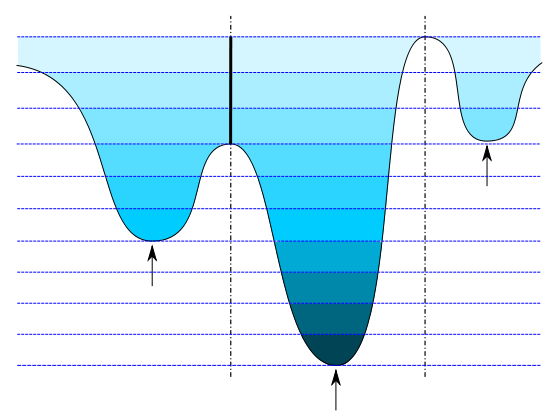
\includegraphics[width=9cm]{imagenes/desarrollo/watershed}
	\caption{El terreno se indica con una línea continua negra, las distintas regiones están marcadas con líneas discontinuas negras, las flechas los mínimos locales, las líneas discontinuas azules los niveles de agua y las líneas discontinuas azules los distintos niveles de agua para realizar la inundación. Imagen extraída de \url{https://en.wikipedia.org/wiki/File:Watershed_transform_-_flood_interpretation.svg}}
	\label{fig:desarrollo/watershed}
\end{figure}

\subsubsection{\textit{Livewire}}

El método de segmentación \textit{livewire} (también conocido como tijeras inteligentes) es, a diferencia de los anteriores, un método basado en bordes.

\textit{Livewire} es un método manual de segmentación donde hace falta la intervención del usuario en prácticamente todo momento pues tiene que ir seleccionando puntos del borde de la región a segmentar en cada corte.

Se hace uso del algoritmo de \textit{Dijkstra} para calcular el camino de coste mínimo entre el punto seleccionado por el usuario y uno anterior. Hace uso de la componente gradiente para dar coste a los nodos del grafo \cite{mortensen95}.

\begin{figure}[H]
	\centering
	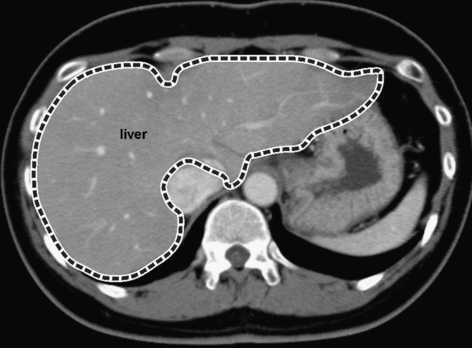
\includegraphics[width=9cm]{imagenes/desarrollo/livewire}
	\caption{Ejemplo de hígado en un corte segmentado usando \textit{livewire} \cite{toennies12}}
	\label{fig:desarrollo/livewire}
\end{figure}

Este método es quizás el más preciso, pero para obtener un resultado hace falta un usuario delante del ordenador recortando todos y cada uno de los cortes del conjunto de datos volumétrico.

\section{Plataforma de desarrollo}

TODO

\subsection{Instalación y configuración}

TODO

\section{Fases de desarrollo}

Inicialmente se planteó un desarrollo en tres partes bien diferenciadas e independientes, aunque una de ellas podría ayudar a lograr mejores resultados en la siguiente. 

Hablo de la de pre-procesamiento de datos (correspondiente a la etapa de filtrado del flujo de representación de datos volumétricos) en la que se marcó el objetivo de reducir el ruido, específicamente el que producían los objetos metálicos. 

Gracias a esto sería más fácil detectar las distintas piezas de madera para la sección de subdivisión de piezas de madera (correspondiente a la etapa de segmentación). 

Por último, ya con estas dos secciones terminadas, se pasaría a añadir herramientas de documentación que ayudarían al restaurador a realizar sus tareas de documentación en la propia aplicación sin necesidad de utilizar herramientas externas.

\subsection{Pre-procesamiento de datos}

El objetivo aquí era la reducción del ruido que se podría encontrar en las imágenes. Como ya se ha explicado anteriormente, hay filtros básicos que nos permiten reducirlo. El filtro media y \textit{gaussiano} nos ayuda a suavizar y el filtro mediana a acabar con \textit{outliers} y ruido de tipo \textit{salt-and-pepper} en general. Aunque en los datos de prueba en los que trabajamos no hay ruido de tipo \textit{salt-and-pepper} es importante proveer este filtro pues en otras imágenes podría haber y es el más efectivo a la hora de acabar con él.

Para no tener que crear las matrices de convolución manualmente \textit{reinventando la rueda}, se hizo uso de una librería que nació precisamente para realizar todas las tareas previas al renderizado de volúmenes y que cuenta con una gama de filtros ya implementados. Hablo de ITK \cite{itk}. Una librería de código abierto de la misma compañía que VTK, \textit{Kitware}.

Esta librería incluye los tres filtros citados con anterioridad:

\begin{itemize}
	\item \textbf{Media}: Usando la clase \texttt{itkMeanImageFilter} pasando como parámetro el tamaño del vecindario.
	\item \textbf{Mediana}: Usando la clase \texttt{itkMedianImageFilter} pasando como parámetro el tamaño del vecindario.
	\item \textbf{\textit{Gaussiano}}: Usando la clase \texttt{itkBinomialBlurImageFilter} pasando como parámetro el número de repeticiones a realizar.
\end{itemize}

Para poder hacer el filtrado hace falta transformar la imagen actual que se encuentra en el formato utilizado en VTK para ser renderizada al formato de ITK. Y una vez realizado el filtro hacer el paso opuesto. Para ello hay que utilizar las clases \texttt{itkVTKImageToImageFilter} e \texttt{itkImageToVTKImageFilter}.

A continuación se presenta un pequeño \textit{script} con los pasos a seguir para realizar el filtrado en una imagen en VTK usando filtros de ITK (Código \ref{code:desarrollo/vtk-itk-filtro}):

\begin{lstlisting}[style=C, label=code:desarrollo/vtk-itk-filtro, caption={\textit{script} para usar el filtro media de ITK en una imagen en VTK}]
// Definir tipo de imagen ITK usando signed short y 3 dimensiones
typedef signed short PixelType;
const unsigned int Dimension = 3;
typedef itk::Image<PixelType,Dimension> ImageType;

// Crear pipeline para pasar una imagen VTK a ITK
typedef itk::VTKImageToImageFilter<ImageType> VTKImageToImageType;
VTKImageToImageType::Pointer vtkImageToImage = VTKImageToImageType::New();
vtkImageToImage->SetInput(imageData);
vtkImageToImage->Update();

// Filtrar la imagen ITK usando un filtro media
typedef itk::MeanImageFilter<ImageType,ImageType> MeanImageFilterType;
MeanImageFilterType::Pointer meanFilter = MeanImageFilterType::New();
meanFilter->SetInput(vtkImageToImage->GetOutput());
meanFilter->SetRadius(radius);
meanFilter->Update();

// Pasara de imagen ITK filtrada a VTK
typedef itk::ImageToVTKImageFilter<ImageType> ImageToVTKImageType;
ImageToVTKImageType::Pointer imageToVTKImage = ImageToVTKImageType::New();
imageToVTKImage->SetInput(meanFilter->GetOutput());
imageToVTKImage->Update();

// Actualizar la instancia de la imagen VTK
imageData->DeepCopy(imageToVTKImage->GetOutput());
imageData->Modified();
\end{lstlisting}

\subsubsection{Integración con la GUI}

La integración con la interfaz es simple e intuitiva. Tan solo hay que pulsar en el botón de filtrado (Figura \ref{fig:desarrollo/gui-filtro}) y aparecerá un cuadro de diálogo donde se podrá elegir el tipo de filtro a aplicar y sus parámetros (Figura \ref{fig:desarrollo/gui-filtro-dialogo}). Una vez seleccionado se pulsa en OK y empezará a filtrar. Es un proceso largo por lo que se coloca un cuadro de diálogo informando al usuario que tenga paciencia.

\begin{figure}[H]
	\centering
	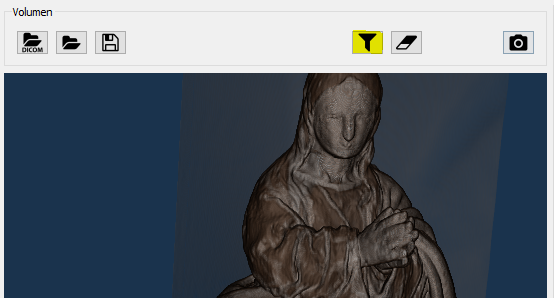
\includegraphics[width=11cm]{imagenes/desarrollo/gui-filtro}
	\caption{Botón que hay que pulsar para que aparezca el diálogo de filtrado}
	\label{fig:desarrollo/gui-filtro}
\end{figure}

\begin{figure}[H]
	\centering
	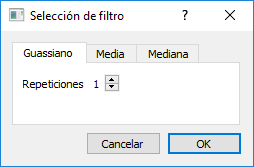
\includegraphics[width=4cm]{imagenes/desarrollo/gui-filtro-gaussiano}
	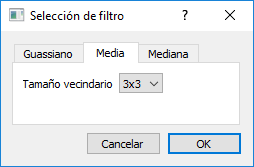
\includegraphics[width=4cm]{imagenes/desarrollo/gui-filtro-media}
	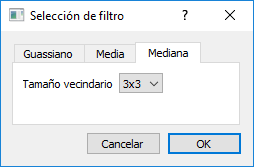
\includegraphics[width=4cm]{imagenes/desarrollo/gui-filtro-mediana}
	\caption{Cuadro de diálogo con los filtros posibles. Se muestran tres imágenes, una por cada pestaña abierta para mostrar el parámetro que hay que establecer para aplicar el filtro}
	\label{fig:desarrollo/gui-filtro-dialogo}
\end{figure}

\subsubsection{Problema con el ruido de elementos metálicos}

Ningún \textit{pipeline} de los filtros citados anteriormente ha ayudado a eliminar el ruido producido por los elementos metálicos (Figura \ref{fig:desarrollo/ruido-clavo}).

\begin{figure}[H]
	\centering
	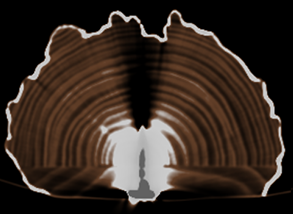
\includegraphics[width=8cm]{imagenes/desarrollo/ruido-clavo}
	\caption{Ruido producido por los elementos metálicos}
	\label{fig:desarrollo/ruido-clavo}
\end{figure}

Y es que ningún filtro estudiado sería capaz de reducir este ruido. Pues el tamaño de vecindario que se debería aplicar sería demasiado grande y suavizaría tanto la imagen que se perderían tantos detalles que no parecería ni la imagen original.

Hay estudios que aseguran haber reducido este ruido en imágenes médicas con pequeños implantes metálicos \cite{deman98} \cite{watzke04}, pero no detallan el comportamiento de su algoritmo para reproducirlo y además, en las imágenes de prueba que utilizan el ruido es ínfimo comparado con el caso de nuestros datos.

Otro estudio más reciente \cite{boas12} usando escáneres más modernos aseguran que retocando los parámetros de este podría eliminarse prácticamente por completo. Por lo que, resolver este problema pasa a ser responsabilidad de la primera fase del flujo del modelado de conjuntos volumétrico, la obtención de datos.

\subsection{Subdivisión de piezas de madera}

El objetivo de esta sección es poder dividir el modelo de una escultura en las distintas piezas de madera que la conforman.

Anteriormente hemos analizado las soluciones que se utilizan actualmente y hemos visto como no son efectivas para resolver nuestro problema. Por tanto, es el momento de proponer e implementar una solución efectiva capaz de separar las distintas piezas de las que está compuesta la escultura.

Para abordar esta situación se va a seguir una de las máximas más importantes a la hora de solucionar problemas, que no es más que dividir el problema en sub-problemas más pequeños. Por lo que, en primer lugar se intentará segmentar una sola imagen y posteriormente aplicar esta solución en todos los cortes del conjunto de datos.

\subsubsection{Segmentación 2D}

Lo primero que tenemos que hacer es preguntarnos a nosotros mismos cómo detectar el cambio entre dos piezas de madera en una escultura. Lo primero que se nos puede ocurrir es que se puede ver un cambio de continuidad en la curvatura de los anillos, pero analizar todos los anillos y realizar un estudio de su continuidad en cada corte puede ser muy costoso y además hay ocasiones en las que el cambio de continuidad no es tan obvio (Figura \ref{fig:desarrollo/continuidad-anillos}).

\begin{figure}[H]
	\centering
	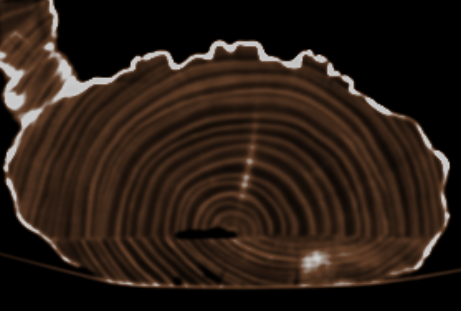
\includegraphics[width=10cm]{imagenes/desarrollo/continuidad-anillos}
	\caption{A la izquierda podemos ver continuidad en algunos anillos}
	\label{fig:desarrollo/continuidad-anillos}
\end{figure}

Tenemos que buscar una solución computacionalmente menos costosa porque tendríamos que lanzar este algoritmo en todos los cortes del conjunto de datos volumétrico y, normalmente, trabajamos con datos de cientos de cortes.

Cuando los escultores ensamblan las piezas de madera que forman el embón de la escultura usan piezas cortadas previamente que encajan y se acoplan más fácilmente. Por tanto el límite entre dos piezas de madera distintas es una línea recta. la detección de este tipo de líneas por un ordenador se puede realizar rápidamente usando técnicas de visión por computador existentes como la transformada de \textit{Hough} \cite{duda72}.

Pero aplicar este algoritmo directamente a una imagen de un corte no nos daría muy buenos resultados si previamente no aplicamos un algoritmo de detección de bordes. Para hacer esto, vamos a usar uno de los más utilizados, el algoritmo de detección de bordes de \textit{Canny} \cite{canny86}. Con este algoritmo y ajustando algunos parámetros podemos obtener con mayor o menor tolerancia los bordes de una imagen (Figura \ref{fig:desarrollo/canny}) que permitiría utilizar de forma más efectiva la transformada de \textit{Hough} para detectar las líneas rectas de la imagen.

\begin{figure}[H]
	\centering
	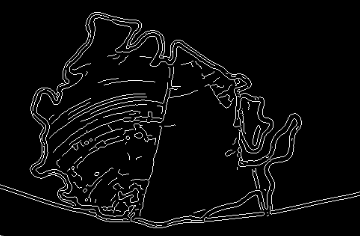
\includegraphics[width=10cm]{imagenes/desarrollo/canny}
	\caption{Corte al que hemos aplicado el algoritmo de detección de bordes de \textit{Canny}. Podemos apreciar fácilmente la línea recta que separa las dos piezas de madera}
	\label{fig:desarrollo/canny}
\end{figure}

Para evitar la generación de algunas líneas producidas por materiales que no son madera, vamos a aplicar previamente un filtro por umbral para quedarnos solo con los datos de la madera. A continuación aplicamos el algoritmo previamente citado de \textit{Hough} para buscar las líneas. 

Las líneas obtenidas las ordenamos de mayor a menor tamaño para descartar líneas rectas que podrían haber anillos o en los bordes de la escultura (Figura \ref{fig:desarrollo/canny-hough}).

\begin{figure}[H]
	\centering
	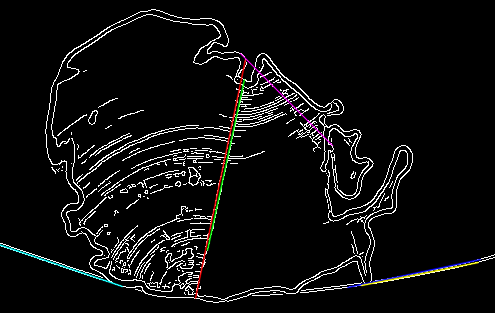
\includegraphics[width=10cm]{imagenes/desarrollo/canny-hough}
	\caption{Corte al que hemos aplicado el algoritmo de detección de bordes de \textit{Canny} para aplicar a continuación el algoritmo de \textit{Hough} para detectar líneas rectas. Se muestran las cinco líneas más largas que se han encontrado}
	\label{fig:desarrollo/canny-hough}
\end{figure}

Una vez tenemos la línea que separa las dos piezas, la segmentación es sencilla porque solo tenemos que aplicar un algoritmo de crecimiento limitado no solo por el umbral, sino por la línea que hemos seleccionado.

Por tanto, para realizar la segmentación en una sola imagen nos hace falta una semilla (la usada en el algoritmo de crecimiento por umbral tradicional) y una línea que limite el crecimiento (Figura \ref{fig:desarrollo/pipeline-segmentacion-2d}).

\begin{figure}[H]
	\centering
	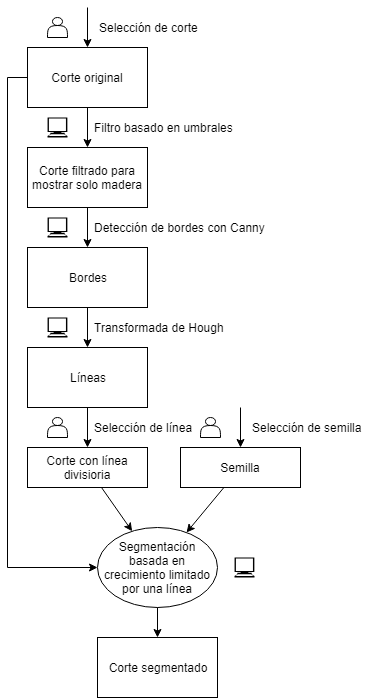
\includegraphics[width=11cm]{imagenes/desarrollo/pipeline-segmentacion-2d}
	\caption{Proceso completo de la segmentación 2D donde se detalla cuándo interviene el ordenador y cuándo lo hace el usuario}
	\label{fig:desarrollo/pipeline-segmentacion-2d}
\end{figure}

\subsubsection{Segmentación 3D}

Para llevar a cabo la segmentación en la totalidad del conjunto de datos volumétrico se realiza la segmentación 2D corte a corte en el eje axial.

Pero como se ha explicado anteriormente, hacen falta tanto la línea que limite la zona de crecimiento como la semilla donde se comience a expandir que no serán los mismos en todos los cortes.

En el caso de la línea es muy difícil que coincida pues rara vez nos encontraremos con un montaje en el que el corte entre las dos piezas forme un ángulo exacto de 90º con respecto al eje axial. Sin embargo, la diferencia entre un corte y otro es milimétrica y la distancia será muy pequeña. Por ello, en lugar de pedir al usuario que elija la línea en cada corte, lo cual sería enormemente tedioso, se realizará una búsqueda de líneas y se escogerá la más cercana a la línea del corte anterior.

Para determinar el criterio de proximidad vamos a utilizar dos factores:

\begin{itemize}
	\item \textbf{Ángulo entre dos líneas}: Dos líneas proyectadas en el mismo plano que forman un ángulo muy pequeño serán muy similares.
	$$ cos(\alpha) = \frac{|u_0 v_0 + u_1 v_1|}{\sqrt{u_0^2 + u_1^2}\sqrt{v_0^2 + v_1^2}} $$
	\item \textbf{Distancia de un punto de una de ellas a la otra}: El ángulo solo no basta. Pues puede que tengan un ángulo muy parecido pero su punto de corte se encuentre muy lejos del espacio que se observa en el visor. Es por ello que hay que tener en cuenta este factor, pues los dos puntos que definen una línea se van a encontrar siempre en el espacio del visor pues es en este donde se lleva a cabo la operación de la búsqueda de líneas rectas y si la distancia mínima de uno de los dos puntos a la otra recta es pequeña significará que las dos líneas se cortan o en el propio espacio que vemos o cerca de éste.
	$$ d(P, r) = \frac{A P_0 + B P_1 + C}{\sqrt{A^2 + B^2}} $$
\end{itemize}

En determinados cortes puede ser que no se observe con suficiente nitidez el borde que separan las dos piezas de madera y por tanto, la transformada de \textit{Hough} no encuentre aquí ninguna línea recta.

Para lidiar con este problema se omitirán este corte y todos los sucesivos donde no encuentre ninguna línea hasta que se de con uno en el que sí. Entonces se trazará un plano que pase por la línea del último corte donde se había encontrado hasta la línea de éste y se utilizará este plano para generar las líneas en todos los cortes intermedios.

Que la semilla de expansión varíe entre corte y corte pasa en menos ocasiones que con la línea pero, a no ser que se trate de una escultura muy regular y se escoja una semilla que sirva para todos los cortes, habrá ocasiones en las que habrá que cambiarla.

Un método que podría servir sería calcular el centroide del área inmediatamente anterior, pero el cálculo de éste es bastante costoso, por lo que, en vez de utilizar el centroide, se utiliza el punto medio: 
$$ M(x,y) = (\frac{x_{min} + x_{max}}{2}, \frac{y_{min} + y_{max}}{2}) $$
que puede ser calculado mientras se está realizando la segmentación.

Como habrá casos en los que este punto medio sea un píxel con un valor escalar fuera de los rangos de valores de madera, por ejemplo podría coincidir con una grieta en ésta, se realizará una expansión (respetando el límite de la línea previamente calculada) hasta encontrar el primer píxel cuyo valor corresponda a la madera para utilizarlo como semilla.

Como podemos ver en los ejemplos (Figura \ref{fig:desarrollo/ejemplos-segmentacion}), se ha creado un método de segmentación semiautomática eficaz con el que poder segmentar dos piezas de madera en un conjunto de datos volumétrico adaptando la segmentación basada en el crecimiento de regiones tradicional para que se vea limitada por una línea que es detectada haciendo uso de técnicas de visión por computador.

\begin{figure}[H]
	\centering
	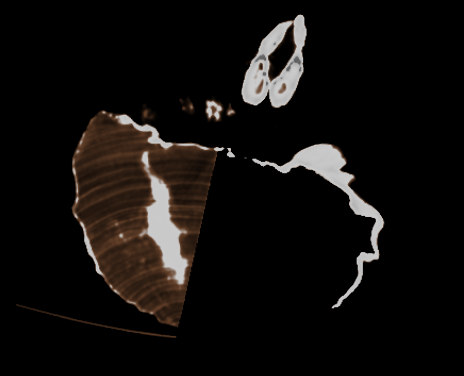
\includegraphics[width=4cm]{imagenes/desarrollo/corte-segmentado-1}
	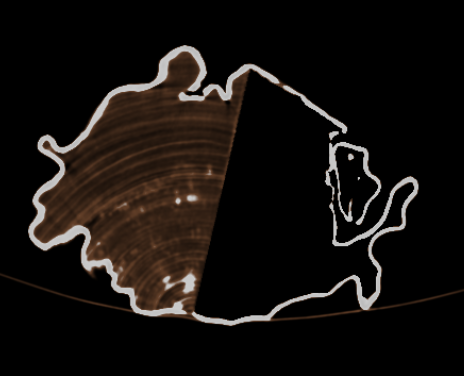
\includegraphics[width=4cm]{imagenes/desarrollo/corte-segmentado-2}
	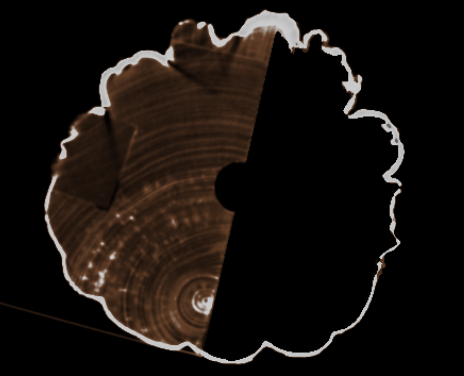
\includegraphics[width=4cm]{imagenes/desarrollo/corte-segmentado-3}
	\caption{Resultado de segmentación en distintos cortes}
	\label{fig:desarrollo/ejemplos-segmentacion}
\end{figure}

Durante todo el proceso, la intervención del usuario solo se da en dos ocasiones: para elegir qué línea utilizar como separadora de piezas y para la selección de la semilla por donde comenzar la expansión.

\subsubsection{Exportar e importar volumen}

Para poder trabajar con el volumen resultado de la segmentación sin tener que segmentarlo todas las veces que se quiera trabajar con él es necesario poder exportarlo a un formato que luego pueda interpretar la aplicación para importarlo.

Se va a utilizar el formato VTI propio de VTK, que utiliza XML para guardar la información del volumen. Para ello hay que hacer uso de las clases \texttt{vtkXMLImageDataWriter} para exportar y \texttt{vtkXMLImageDataReader} para importar.

Además, gracias al uso de este tipo de archivo, se puede reducir bastante el tamaño de los archivos con datos volumétricos. Los datos en crudo en formato DICOM de una de las esculturas ocupan 236MB, mientras que esos mismos datos extraídos a formato VTI pasan a ocupar casi la mitad, 128MB.

\subsubsection{Integración con la GUI}

Para integrarlo con la interfaz gráfica se ha hecho algo parecido a lo que se hizo con la parte de borrar partes. Se puede activar un modo de segmentación que cambia el interactor del visor de cortes para que atienda al evento del click izquierdo del ratón para usar el píxel clickado como semilla (Figura \ref{fig:desarrollo/gui-segmentacion}).

\begin{figure}[H]
	\centering
	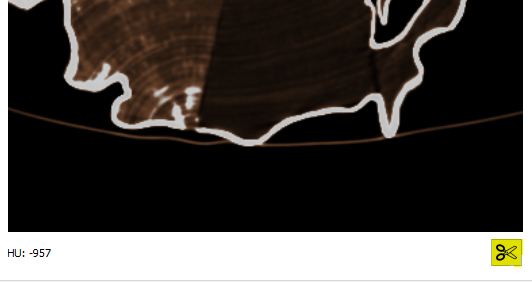
\includegraphics[width=11cm]{imagenes/desarrollo/gui-segmentacion}
	\caption{Botón que hay que pulsar para cambiar a modo de segmentación}
	\label{fig:desarrollo/gui-segmentacion}
\end{figure}

A continuación se pasarán a detectar las líneas rectas de ese corte y se le mostrará una ventana al usuario donde elegirá la línea que quiere utilizar como semilla y si quiere que se fuerce hacia arriba y hacia abajo la segmentación (Figura \ref{fig:desarrollo/gui-segmentacion-linea}). Si no se seleccionan estas opciones, si se deja de encontrar líneas coincidentes con la semilla en cortes superiores o inferiores no se forzará el crecimiento en estos cortes.

\begin{figure}[H]
	\centering
	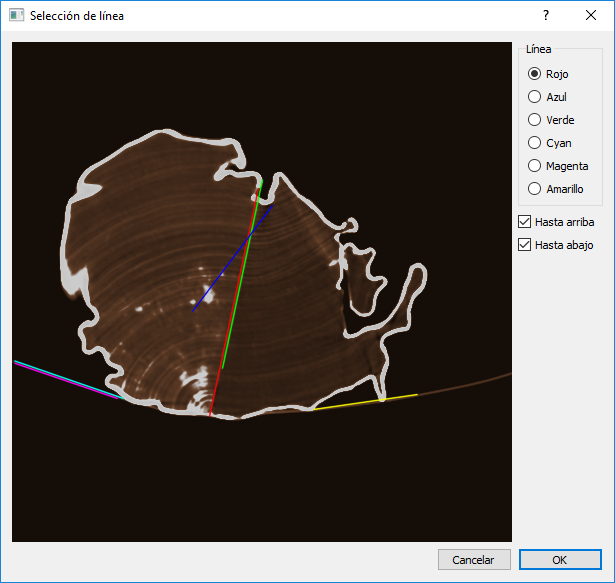
\includegraphics[width=11cm]{imagenes/desarrollo/gui-segmentacion-linea}
	\caption{Líneas detectadas en el corte. El usuario tiene que elegir cuál quiere utilizar}
	\label{fig:desarrollo/gui-segmentacion-linea}
\end{figure}

Una vez seleccionados estos parámetros pasará a segmentar la pieza y al acabar mostrará otra ventana con el volumen resultado para preguntar al usuario si lo quiere o no exportar.

\begin{figure}[H]
	\centering
	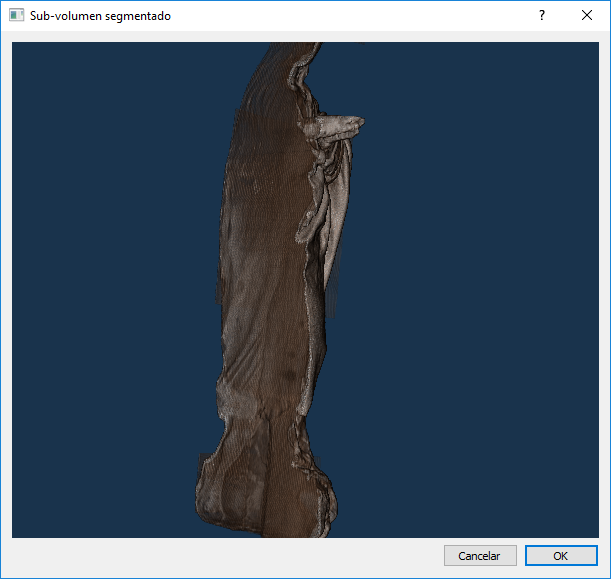
\includegraphics[width=11cm]{imagenes/desarrollo/gui-segmentacion-resultado}
	\caption{Resultado de la segmentación, si se pulsa en OK se pasará a guardar}
	\label{fig:desarrollo/gui-segmentacion-resultado}
\end{figure}

\subsection{Herramientas de documentación}

Hasta ahora, el usuario ha podido analizar la escultura, pero todas las anotaciones las ha debido hacer a parte en una libreta o un documento digital. Lo complicado está en cuando ha tenido que colocar el plano en una posición extraña a la hora de encontrar un artefacto de interés. ¿Cómo lo vuelve a colocar así cuando abra de nuevo el programa? O más complicado todavía, ¿cómo lo pone un compañero que también esté trabajando en esa figura?

Es necesario poder proveer a la aplicación de funcionalidad para poder guardar anotaciones y dónde las ha encontrado para poder continuar con el trabajo en distintas sesiones.

\subsubsection{ROD}

Se ha creado un término, ROD (que viene de las siglas del inglés \textit{Region of Documentation}), que no es más que la posición de un plano en una figura donde realizar anotaciones.

Para crearlo, el usuario tan solo tiene que colocar el plano en la posición deseada y añadir una ROD (Figura \ref{fig:desarrollo/gui-rod}).

\begin{figure}[H]
	\centering
	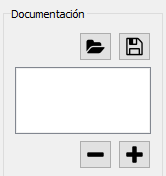
\includegraphics[width=4cm]{imagenes/desarrollo/gui-rod}
	\caption{Listado de ROD y acciones para realizar con ellas}
	\label{fig:desarrollo/gui-rod}
\end{figure}

Al crear la ROD se le pedirá darle un nombre, y si no se proporciona ningún nombre se le pone uno por defecto.

Una vez esté la ROD creada, si el usuario mueve el plano de corte y quiere volver al plano de corte que había guardado, solo tiene que pulsar en el dentro de la lista de ROD.

Si se ha equivocado o ya no lo necesita lo puede borrar utilizando el botón específico para ello.

\subsubsection{Reglas}

La herramienta de las reglas ya se creó anteriormente en el TFG usando el \textit{widget} de VTK \texttt{vtkDistanceWidget}. Sin embargo, al introducir este nuevo concepto de ROD, hay que adaptarlo para que, las reglas creadas no pertenezcan a un espacio global si no a una ROD específica. De esta forma, al mover el plano estas medidas, que ya dejan de tener sentido, desaparecen y puedes volver a verlas seleccionando de nuevo la ROD a la que pertenecen.

Las acciones a realizar son: añadir, eliminar y ocultar/mostrar (Figura \ref{fig:desarrollo/gui-reglas}).

\begin{figure}[H]
	\centering
	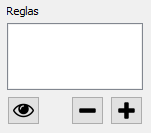
\includegraphics[width=4cm]{imagenes/desarrollo/gui-reglas}
	\caption{Listado de reglas y acciones para realizar con ellas}
	\label{fig:desarrollo/gui-reglas}
\end{figure}

Al añadir una nueva regla habrá que seleccionar los puntos inicial y final que se quieren medir y se mostrará la medida real en milímetros. No hay límite de reglas, por lo que se pueden crear tantas como se quieran. Si se quiere editar tan solo hay que seleccionar y mover uno de los puntos.

\subsubsection{Transportadores de ángulos}

Otra funcionalidad útil parecida a la de medir distancias es medir ángulos. Además, VTK también proporciona un \textit{widget} para realizar esta tarea: \texttt{vtkAngleWidget}. El funcionamiento con los ángulos es exactamente el mismo que el de las reglas. Pertenecen a una ROD, se pueden añadir tantos como se quieran y se pueden eliminar y ocultar/mostrar (Figura \ref{fig:desarrollo/gui-angulos}).

\begin{figure}[H]
	\centering
	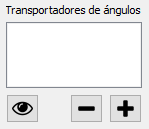
\includegraphics[width=4cm]{imagenes/desarrollo/gui-angulos}
	\caption{Listado de transportadores de ángulos y acciones para realizar con ellos}
	\label{fig:desarrollo/gui-angulos}
\end{figure}

Para añadir un nuevo transportador de ángulos hay que seleccionar tres puntos en este orden: desde dónde, centro y hasta dónde. El resultado será el ángulo formado en grados. Para editarlo solo hay que seleccionar y mover cualquiera de sus puntos.

\subsubsection{Notas}

Además de medir distancias y ángulos, una de las tareas más utilizadas por un restaurador a la hora de examinar una escultura es realizar anotaciones de texto. Para realizar esta tarea se usará otro \textit{widget} de VTK creado para ello, \texttt{vtkCaptionWidget} y se podrán realizar las mismas acciones que con reglas y ángulos (Figura \ref{fig:desarrollo/gui-notas}).

\begin{figure}[H]
	\centering
	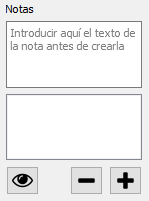
\includegraphics[width=4cm]{imagenes/desarrollo/gui-notas}
	\caption{Listado de notas y acciones para realizar con ellas}
	\label{fig:desarrollo/gui-notas}
\end{figure}

La diferencias con respecto a las anteriores es que antes de crearla hay que introducir en un cuadro de texto el contenido de ella. Esto creará el objeto y el usuario tendrá que mover la flecha a donde apunta.

\subsubsection{Exportar e importar ROD}

TODO

\subsection{Internacionalización}

Una vez terminadas el resto de secciones se pasó a realizar una tarea que acabó resultando tediosa por culpa de no haberla hecho desde un principio. Hablo de la internacionalización: preparar la aplicación para poder traducirla a distintos idiomas. Hasta ahora se tenían todos los textos \textit{hard-coded}, se ha pasado a usar claves y dar los valores a esos claves en una archivo por idioma con el formato TS de Qt.

Una vez rellenos estos archivos hay que compilarlos a formato QM con la herramienta \texttt{lrelease} que proporciona Qt y leer este archivo en el \texttt{main} usando la función \texttt{load()} de \texttt{QTranslator}. Para que los archivos sean accesibles desde la aplicación hay que añadirlos como recursos en un archivo QRC como ya se hace con las imágenes, los iconos y los \textit{presets}.

Con estos cambios se puede generar un ejecutable en español e inglés. Con la posibilidad de añadir otros idiomas fácilmente traduciendo los títulos al idioma que se quiere traducir en un nuevo archivo TS, que se compila a QM, se añade al archivo de recursos QRC y se lee con la función \texttt{load()} de \texttt{QTranslator}.